\section{Klassifizierungsgenauigkeit der Standorte}
Die Klassifizierungsgenauigkeit der ML-Modelle zur Standorterkennung wurde mit verschiedenen Konfigurationen über komplexer werdende Datenmengen evaluiert.
In Kapitel \ref{sec:model_dt} und Kapitel \ref{sec:model_ffnn} werden die einzelnen Konfigurationen der ML-Modelle beschrieben.
Die Komplexität wird über die Anzahl der Standorte definiert.
Um die Anzahl der Standorte zu erhöhen, wurden die Datenmengen um weitere Routen erweitert.
Dies impliziert aber, dass die Testmengen nicht vergleichbar sind unter den verschiedenen Standortkomplexitäten, da mit jeder Route die Testmenge erweitert wird.
Die berechneten Klassifizierungswahrscheinlichkeiten sind jeweils der Durchschnitt der Klassifizierungswahrscheinlichkeiten aller Routen in der Testmenge.
\newline
\newline
Außerdem unterscheiden sich die Enkodierungsansätze je nach Standortkomplexität.
Für die Standortkomplexitäten 9, 17, 25 und 52 wurde der Kodierungsansatz verwendet, bei denen nur die Knoten und ein zusätzlicher unbekannter Standort betrachtet wird.
Für die Standortkomplexitäten 16, 32, 48 und 102 wurde der Kodierungsansatz verwendet, bei denen Knoten und Kanten betrachtet werden.
Ein besserer Ansatz, um Daten mit beliebiger Komplexität zu generieren wird in Kapitel \ref{chapter:discussion} diskutiert.
\newline
\newline
Zunächst wird die Klassifizierungsgenauigkeit $P(A)$ im Vergleich zu Mians Ergebnissen betrachtet.
Mian konnte mit einem WFFNN bei einer Route mit drei Pfaden und 14 Standorten eine Klassifizierungsgenauigkeit von 94,1\% erreichen \cite{naveedThesis}.
Abbildung \ref{fig:best_dt_acc_vs_knn_acc_vs_cont} vergleicht die Klassifizierungsgenauigkeiten der
Entscheidungsbaum basierten Klassifizierer und FFNN über verschiedene Standortkomplexitäten.
Dabei wurde stets die höchste Klassifizierungsgenauigkeiten aller evaluierten Konfigurationen ausgewählt.
Gezeigt werden sowohl die Klassifizierungsgenauigkeiten auf die Testmengen die korrekt beschriftet sind und die, die von den ML-Modellen beschriftet sind.
\begin{figure}[h!]
    \centering
    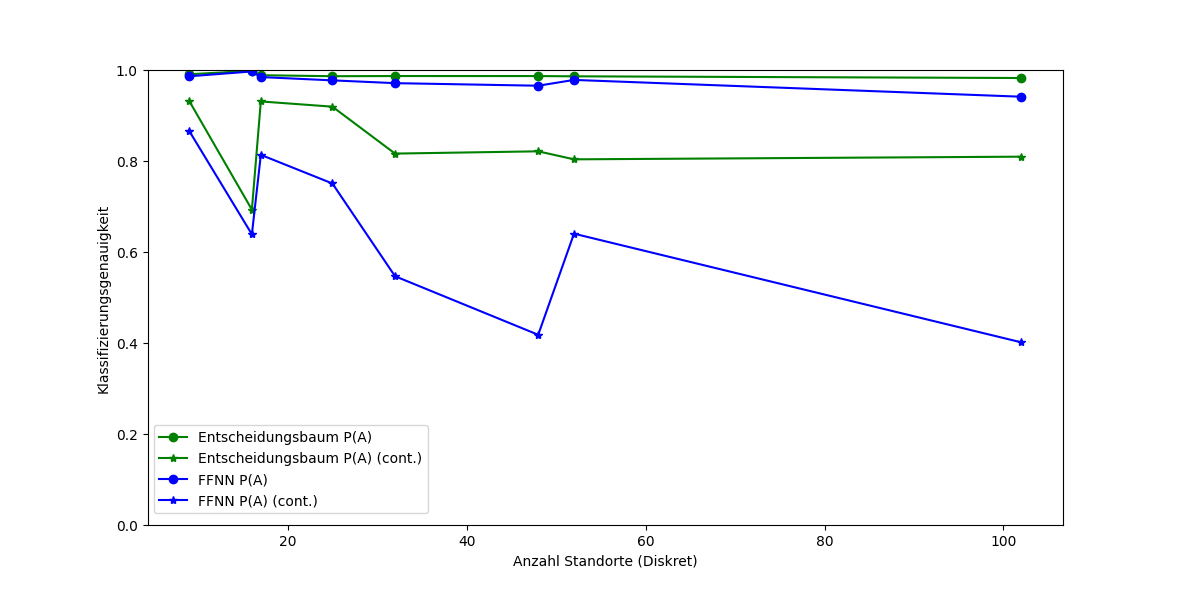
\includegraphics[width=\linewidth]{images/best_dt_vs_knn_acc_vs_acc_cont.png}
    \caption{Die besten Klassifizierungsgenauigkeiten aller evaluierten Konfigurationen der ML-Modelle über alle Standortkomplexitäten.}
    \label{fig:best_dt_acc_vs_knn_acc_vs_cont}
\end{figure}
\newline
\newline
Mian hat in seiner Evaluation die Klassifizierungsgenauigkeit $P(A)$ betrachtet.
Die in dieser Arbeit evaluierten Standortkomplexität, die Mians Evaluation am nächsten kommt ist 16.
Im Vergleich ist der beste Entscheidungsbaum basierte Klassifizierer mit einer Klassifizierungsgenauigkeit von 99,9\%, 5,8 Prozentpunkte besser
und das beste FFNN mit einer Klassifizierungsgenauigkeit von 99,79\%, 5,69 Prozentpunkte besser (Tabelle \ref{tab:predictions_by_acc}).
\newline
\newline
Dies betrachtet aber nicht den propagierten Fehler, der durch die Rekurrenz der ML-Modelle durch die Rückwärtskante entsteht.
In Abbildung \ref{fig:best_dt_acc_vs_knn_acc_vs_cont} ist zu sehen, dass die Klassifizierungsgenauigkeit signifikant geringer ist bei allen Standortkomplexitäten,
wenn die Features für die vorherigen Positionen iterativ bestimmt werden ($P(A)_{\text{cont}}$).
Insbesondere die Standortkomplexität 16 hat eine signifikant geringere Klassifizierungsgenauigkeit, wobei dies eine Artefakt der Enkodierungsmethode sein kann,
da bei der Standortkomplexität 17 immernoch Entscheidungsbaum basierte Klassifizierer mit einer Klassifizierungsgenauigkeit von 94,41\% gefunden wurden (Tabelle \ref{tab:predictions_by_acc_cont}).
Die FFNNS hingegen erreichen lediglich maximal 87,22\% bei dieser Standortkomplexität.
\newline
\newline
Aus Tabelle \ref{tab:predictions_by_acc_10_cont} können die Klassifizierungsgenauigkeiten $P(B=10)$ entnommen werden.
Der Entscheidungsbaum basierte Klassifizierer skaliert dabei sehr gut mit der steigenden Standortkomplexität.
Aber einer Standortkomplexität von 32 wird konnte aber nurnoch eine Klassifizierungsgenauigkeit von 91,35\% erreicht werden, die bis auf 87,87\% bei 102 Standorten fällt.
Als beste maximale Baumhöhe hat sich 16 herausgestellt, wobei 32 und 64 marginal schlechtere Ergebnisse produzierten.
Eine maximale Baumhöhe von 8 war nicht ausreichend, da es für hohe Standortkomplexitäten schlechtere Ergebnisse erzielt hat.
Bei gleicher Waldgröße haben die maximalen Baumhöhen und 32 und 64 equivalente Ergebnisse produziert,
d. h. für die evaluierten Szenarien wird nicht mehr als eine maximale Baumhöhe von 32 benötigt.
Dies schließt aber nicht aus, dass andere Szenarien nicht von größeren maximalen Baumhöhen profitieren könnten.
Die verschiedenen Waldgrößen unterscheiden sich nicht stark.
Eine Waldgröße von 8 hat nur marginal schlechtere Ergenisse bei 102 Standorten erzielt, als die Waldgrößen 16, 32 und 64.
Aus diesem Grund ist eine Waldgröße von 8 ausreichend, oder könnte womöglich reduziert werden.
\begin{table}[h!]
    \hspace{-2cm}
    \begin{tabular}{ | c | c | c | c | c | c | c | c | c | c | }
        \hline
        \multicolumn{2}{ | l |}{$P(B=10)_{\text{cont}}$ über Standorte} & 9 & 16 & 17 & 25 & 32 & 48 & 52 & 102 \\\hline
        \multicolumn{10}{| l |}{\textbf{Entscheidungswälder}}\\\hline
        Waldgröße & Max. Baumgröße & \multicolumn{8}{ c |}{}\\\hline
        16 & 8 & 99.75\% & 81.69\% & 99.68\% & 96.97\% & 82.88\% & 84.28\% & 86.21\% & 79.01\% \\\hline
        16 & 16 & 99.06\% & 77.30\% & 99.09\% & 97.17\% & 91.35\% & 89.01\% & 86.01\% & 89.10\% \\\hline
        16 & 32 & 99.51\% & 77.00\% & 98.55\% & 97.86\% & 86.55\% & 87.05\% & 88.73\% & 85.69\% \\\hline
        16 & 64 & 99.51\% & 77.00\% & 98.55\% & 97.86\% & 86.55\% & 87.05\% & 88.73\% & 85.69\% \\\hline
        8 & 32 & 99.20\% & 92.79\% & 99.67\% & 97.89\% & 90.27\% & 91.01\% & 91.59\% & 85.11\% \\\hline
        32 & 32 & 99.50\% & 78.06\% & 99.65\% & 97.70\% & 88.83\% & 88.31\% & 88.24\% & 86.92\% \\\hline
        64 & 32 & 99.58\% & 84.66\% & 99.51\% & 97.45\% & 89.65\% & 89.59\% & 86.96\% & 87.87\% \\\hline
        32 & 64 & 99.50\% & 78.06\% & 99.65\% & 97.70\% & 88.83\% & 88.31\% & 88.24\% & 86.92\% \\\hline
        \multicolumn{10}{| l |}{\textbf{Feed Forward neuronale Netzwerke}}\\\hline
        \#Schichten & \#Neuronen & \multicolumn{8}{ c |}{}\\\hline
        1 & 16 & 98.70\% & 76.69\% & 92.81\% & 80.31\% & 45.93\% & 46.61\% & 75.48\% & 42.39\% \\\hline
        1 & 32 & 97.82\% & 77.04\% & 92.02\% & 83.61\% & 63.63\% & 47.25\% & 74.30\% & 44.73\% \\\hline
        1 & 64 & 95.53\% & 68.52\% & 92.42\% & 86.31\% & 50.44\% & 40.67\% & 75.80\% & 33.87\% \\\hline
        1 & 128 & 98.11\% & 75.39\% & 95.15\% & 86.21\% & 52.27\% & 32.42\% & 78.92\% & 42.56\% \\\hline
        2 & 32 & 98.67\% & 63.99\% & 90.59\% & 83.71\% & 68.52\% & 34.81\% & 74.03\% & 35.48\% \\\hline
        4 & 32 & 95.14\% & 71.53\% & 89.49\% & 80.25\% & 49.47\% & 27.07\% & 71.79\% & 38.66\% \\\hline
        8 & 32 & 92.94\% & 62.31\% & 90.45\% & 82.21\% & 36.36\% & 35.73\% & 74.55\% & 51.15\% \\\hline
        4 & 64 & 94.88\% & 67.74\% & 89.91\% & 84.34\% & 54.47\% & 23.57\% & 75.18\% & 47.55\% \\\hline
    \end{tabular}
    \caption{Metrik $P(B=10)_{\text{cont}}$ über Standorte und verschiedenen Konfigurationen der ML-Modelle.}
    \label{tab:predictions_by_acc_10_cont}
\end{table}
\newline
\newline
Die evaluierten FFNNs skalieren deutlich schlechter als die Entscheidungsbaum basierten Klassifizierer mit steigender Standortkomplexität.
Insbesondere die FFNNs der Standortkomplexitäten, die das Enkodierungsverfahren der Kanten und Knoten nutzten,
konnten signifikant schlechtere Klassifizierungsergebnisse erzielen als die FFNNs die nur die Knoten kodierten.
Aus den Daten ist nicht zu schließen, wie sich die Anzahl der Schichten und Neuronen pro Schicht auf die Klassifizierungsgenauigkeit auswirkt.
Große FFNNs wirken im Vergleich zu kleinen FFNNs aber sehr volatil, d. h. sie können sowohl deutlich bessere Ergebnisse als die kleinen FFNNs erzielen, aber auch deutlich schlechtere Ergebnisse.
\newline
\newline
Sowohl bei den Entscheidungswäldern, als auch bei den FFNNs, ist eine geringere Klassifizierungsgenauigkeit mit dem Kodierungsansatz der Kanten und Knoten enkodirt
zu beobachten, als mit dem Kodierungsansatz der nur die Knoten kodiert.
Insbesondere zwischen den Standortkomplexitäten 16 und 17, sowie 32, 48 und 52 ist diese Diskrepanz zu erkennen.
Aus diesem Grund ist zu schließen, dass der Kodierungsansatz, der nur Knoten kodiert, besser skaliert, als der Kodierungsansatz, der Kanten und Knoten kodiert.